
\section{Dust waves in the drag-free limit}
\label{sec:gas-free-bow}

% As an alternative to hydrodynamic or magnetohydrodynamic bow shocks,
% it is possible that some observed emission arcs may be bow waves due
% to the action of radiation pressure on dust grains.

\begin{figure}
  (a)\\
  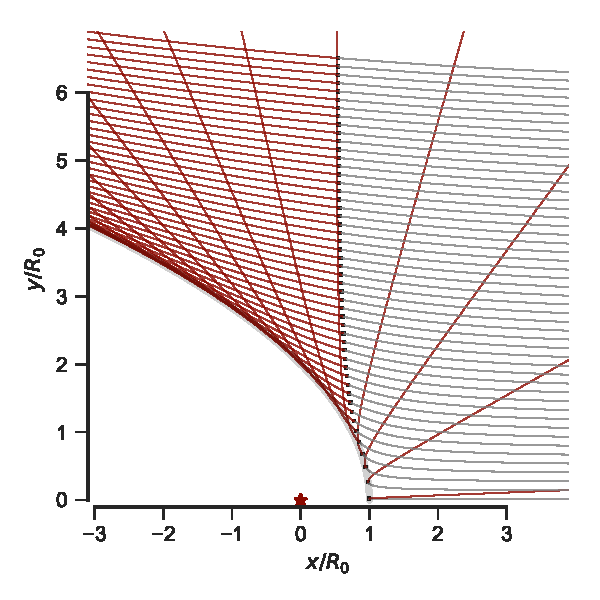
\includegraphics[width=\linewidth]{figs/dust-trajectories}
  (b)\\
  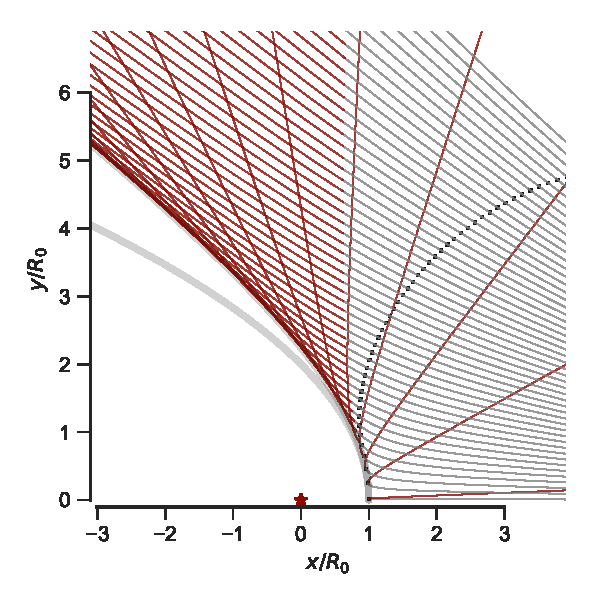
\includegraphics[width=\linewidth]{figs/dust-divergent}
  \caption[Dust grain trajectories]{Dust grain trajectories under
    influence of a repulsive central \(r^{-2}\) radiative force.
    (a)~A parallel stream of dust grains approach from the right at a
    uniform velocity and with a variety of impact parameters (initial
    \(y\)-coordinate). The central source is marked by a red star at
    the origin, and its radiative force deflects the trajectories into
    a hyperbolic shape, each of which reaches a minimum radius marked
    by a small black square.  The incoming hyperbolic trajectories are
    traced in gray and the outgoing trajectories are traced in red.
    The locus of closest approach of the outgoing trajectories is
    parabolic in shape (traced by the thick, light gray line) and this
    constitutes the inner edge of the bow wave.  (b)~The same but for
    a divergent stream of dust grains that originates from a source on
    the \(x\) axis at a distance \(D = 10 R\starstar\) from the
    origin.  In this case, the inner edge of the bow wave is
    hyperbolic and the parallel stream result is also shown (inner
    thick light gray line) for comparison.}
  \label{fig:dust-trajectories}
\end{figure}



In the optically thin limit, a spherical dust grain of radius \(a\)
situated a distance \(R\) from a point source of radiation with
luminosity spectrum \(L_\nu\) will experience a repulsive, radially
directed radiative force \citep[e.g.,][]{Spitzer:1978a}
\begin{equation}
  \label{eq:dust-rad-force}
  \frad = \frac{\pi a^2 } {4 \pi R^2 c}  \int_0^\infty \Qp \, L_\nu \, d\nu 
\end{equation}
where \Qp{} is the frequency-dependent radiation pressure efficiency\footnote{%
  \label{fn:Qp}
  For absorption efficiency \(Q_{\text{abs}}\), scattering efficiency
  \(Q_{\text{scat}}\), and asymmetry parameter (mean scattering
  cosine) \(g\), we have
  \(\Qp = Q_{\text{abs}} + (1 - g) Q_{\text{scat}}\) \citep[e.g.,
  \S~4.5 of][]{Bohren:1983a}.} %
of the grain, and \(c\) is the speed of light.

% \subsection{Gas-free dust wave}

If \(\frad\) is the only force experienced by the grain, then it will
move on a \textit{ballistic} trajectory, determined by its initial
speed at large distance, \(v_\infty\), and its impact parameter, \(b\).
For \(b = 0\), the grain radially approaches the source with initial
radial velocity \(-v_\infty\), which is decelerated to zero at the distance
of closest approach, \(R\starstar\), given by energy conservation:
\begin{equation}
  \label{eq:dust-r0}
  R\starstar = \frac{\kappa\grain L} {2 \pi c v_\infty^2} \ ,
\end{equation}
where we have defined a frequency-averaged single-grain opacity
(\si{cm^2.g^{-1}}) as
\begin{equation}
  \label{eq:kappa-grain}
  \kappa\grain = \frac{\pi a^2}{m\grain L} \int_0^\infty \Qp \, L_\nu \, d\nu \ ,
\end{equation}
in which \(m\grain\) is the grain mass and \(L\) is the bolometric
source luminosity.  The grain then turns round and recedes from the
source along the same radius, reaching a velocity of \(+v_\infty\) at large
distance.  Note that \(R\starstar\) as given by
equation~\eqref{eq:dust-r0} is formally identical to Paper~I's
equation~(6), but with the important difference that it is for a
single grain considered in isolation, rather than a well-coupled dusty
plasma.  If 

For \(b > 0\), the problem is formally identical to that of Rutherford
scattering, or (modulo a change of sign) planetary orbits.  The method
of solution (via introduction of a centrifugal potential term and
reduction to a 1-dimensional problem) can be found in any classical
mechanics text \citep[e.g.,][\S~14]{Landau:1976a}.  The trajectory,
\(R\grain(\theta; b)\), is found to be hyperbolic, characterized by an
eccentricity,
\(\varepsilon = \bigl( 1 + 4 b^2 / R\starstar^2\bigr)^{1/2}\), and polar angle
of closest approach, \(\thm = \cos^{-1} \varepsilon^{-1}\).  The trajectory is
symmetrical about \(\thm\) and can be written as
\begin{equation}
  \label{eq:dust-r-theta}
  \frac{R\grain(\theta; b)} {R\starstar} = 
  \frac{ \tfrac12 \bigl( \varepsilon^2 - 1 \bigr)} {\varepsilon \cos(\theta - \thm) - 1} \ , 
\end{equation}
with a total deflection angle of \(\ang{180} - 2 \thm\), which is equal to
\ang{90} when \(b = 0.5 R\starstar\).

\subsection{Parallel dust stream}
\label{sec:dust-parallel}

If the incoming dust grains initially travel along parallel
trajectories with varying \(b\), but the same \(v_\infty\), then deflection
by the radiative force will form a bow-shaped dust wave around the
radiation source, as shown in Figure~\ref{fig:dust-trajectories}.
However, the inner edge of the dust wave, \(R_{\text{in}}(\theta)\) is not
given by the closest approach along individual trajectories,
\(R\grain(\thm; b)\), but instead must found by minimizing
\(R\grain(\theta; b)\) over all \(b\) for each value of \(\theta\), which yields
\begin{equation}
  \label{eq:dust-r-in}
  \frac{R_{\text{in}}(\theta)} {R\starstar} = \frac{2}{1 + \cos\theta} \ .
\end{equation}
This is the polar form of the equation for the confocal parabola,
which we have already discussed in detail in \S~\ref{Q-sec:conic} and
Appendix~\ref{Q-app:parabola} of \citet{Tarango-Yong:2018a}.  Its
planitude and alatude are \(\Gamma = \Lambda = 2\) and these are
unchanged under projection at any inclination.



\subsection{Divergent dust stream}
\label{sec:dust-divergent}

If the dust grains are assumed to originate from a second point
source, located at a distance \(D\) from the radiation source, then
the incoming stream will be divergent instead of plane parallel.  The
individual streamlines are not affected by this change and are still
described by equation~\eqref{eq:dust-r-theta}, except that the
trajectory axes for \(b > 0\) are no longer aligned with the global
symmetry axis, so we must make the substitution
\(\theta \to \theta + \theta_1(b)\), where \(\sin \theta_1 = b / D\) (see
Fig.~\ref{Q-fig:crw-schema} of \citealp{Tarango-Yong:2018a}). We
parameterize the degree of divergence as \(\mu = R\starstar / D\) and, as
before, \(R\grain(\theta + \theta_1(b, \mu); b)\) is minimized over all
trajectories to find the shape of the bow wave's inner edge.  This
time, the result is a confocal hyperbola:
\begin{equation}
  \label{eq:dust-divergent-r-in}
  \frac{R_{\text{in}}(\theta; \mu)} {R\starstar} = \frac{1 + \varepsilon_\mu}{1 + \varepsilon_\mu\cos\theta} \ ,
\end{equation}
where the eccentricity is (to first order in \(\mu\))
\( \varepsilon_\mu = (1 - 2\mu)^{-1}\).  An example is shown in
Figure~\ref{fig:dust-trajectories} for \(\mu = 0.1\).  Unsurprisingly,
the resulting bow shape is more open than in the parallel stream case,
increasingly so with increasing \(\mu\).  The planitude and alatude are
both equal: \(\Pi = \Lambda = 1 + \varepsilon_\mu\).

\subsection{Magnetized dust waves}
\label{sec:tight-magn-coupl}

\begin{figure}
  \centering
  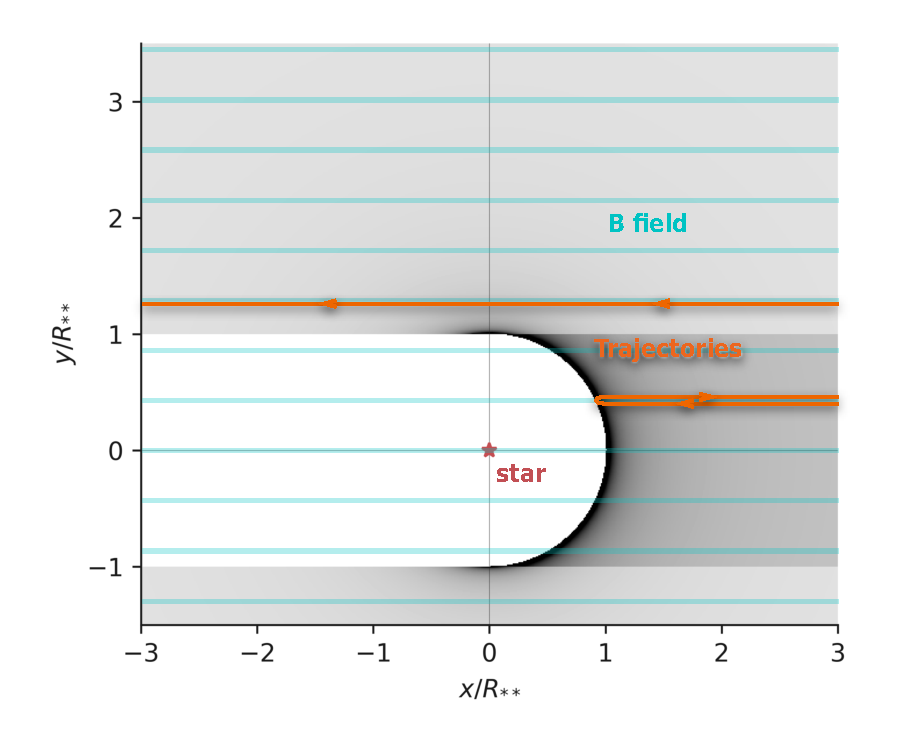
\includegraphics[width=\linewidth]{figs/parallel-bfield-dust-wave-inertia}
  \caption{Dust wave formed by action of radiation forces on grains
    that are tightly coupled to a uniform parallel magnetic field.
    Two example trajectories, one with \(b > R\starstar\) (upper) and
    one with \(b < R\starstar\) (lower) are shown schematically in
    orange.  The orientation of the magnetic field lines is shown in
    blue.  The grayscale image shows the resultant dust density
    distribution.}
  \label{fig:inertia-thB0}
\end{figure}

\begin{figure}
  \centering
  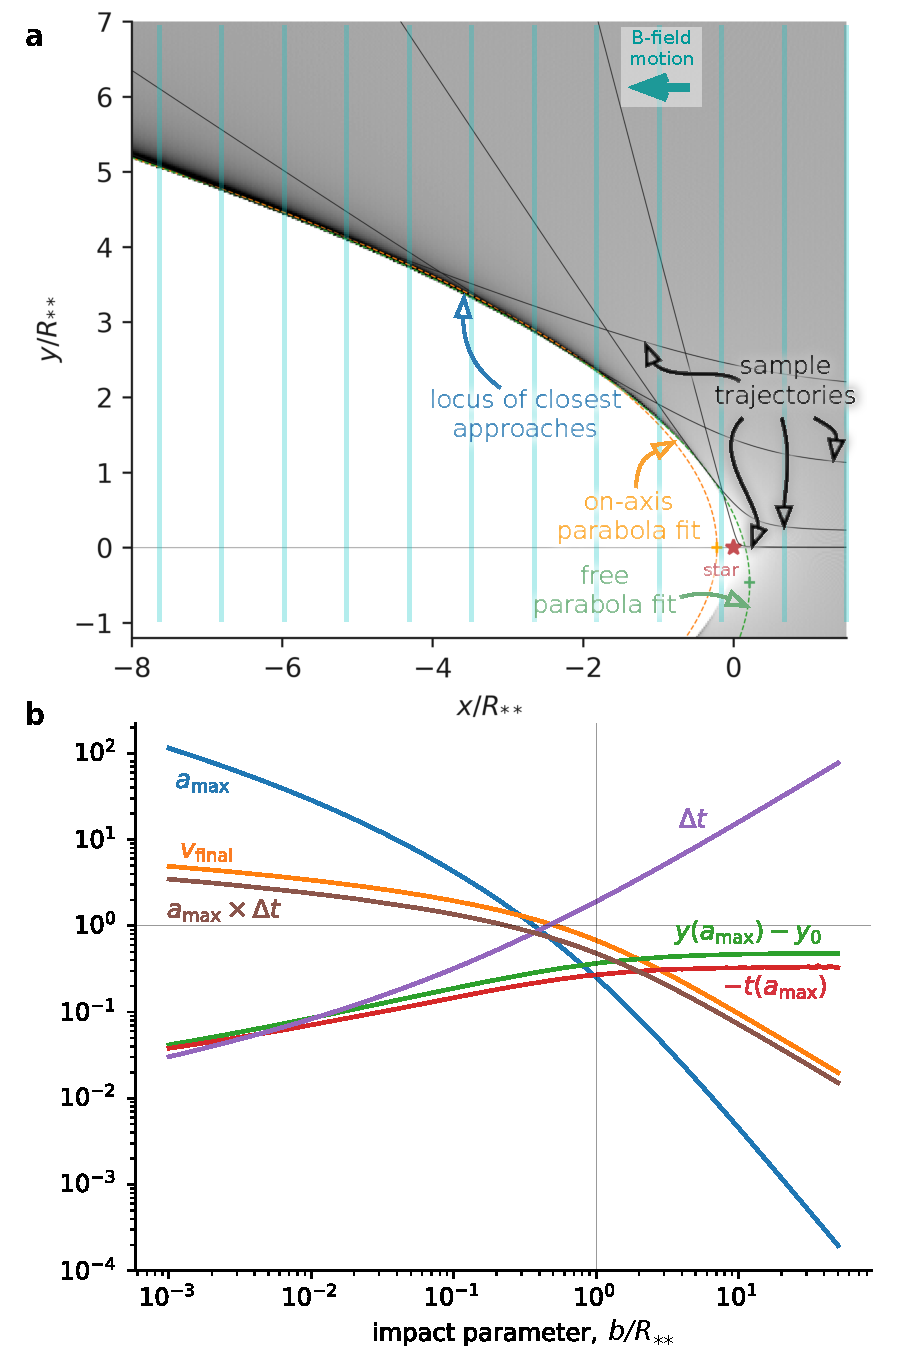
\includegraphics[width=\linewidth]{figs/perp-bfield-dust-wave-inertia}
  \caption{Dust wave formed by action of radiation forces on grains
    that are tightly coupled to a uniform perpendicular magnetic
    field.  (a)~Sample trajectories are shown by thin black lines and
    the resultant dust density distribution in grayscale.  Two
    parabolic fits to the inner edge of the dust wave in the wing
    region (\(y > R\starstar\)) are shown. The orange line shows a
    simultaneous fit to both wings, while the green line shows a fit
    to a single wing, in which the parabola apex is not constrained to
    lie on the axis.  The second fit has much smaller residuals,
    indicating that the overall dust wave shape is ``pointier'' than a
    parabola, but this is hard to quantify because the disappearance
    of the dense shell in the apex region makes it impossible to
    define \(R_0\) for the bow.  (b)~Trajectory parameters over a wide
    range of impact parameters, shown on a log--log scale. Distances
    are in units of \(R\starstar\), times in units of
    \(R\starstar / v_\infty\), velocities in units of \(v_\infty\), and
    accelerations in units of \(v_\infty^2 / R\starstar\). The grain's
    acceleration along the \(y\) axis has a maximum value,
    \(a_{\text{max}}\), which occurs at a position
    \(x(a_{\text{max}}), y(a_{\text{max}})\), just before the grain is
    swept past the star, with a duration (FWHM) of \(\Delta t\).  The
    grain's asymptotic \(y\) velocity is \(v_{\text{final}}\) and the
    fact that this closely tracks \(a_{\text{max}} \times \Delta t\) indicates
    that the majority of the acceleration occurs in a sharp impulse.
    The curves tend to straight lines at the right side of the graph,
    which gives the asymptotic scaling relations discussed in the
    text.}
  \label{fig:inertia-thB90}
\end{figure}

We will show later in \S~\ref{sec:magn-effects-grain} that for
sufficiently small grains the Larmor magnetic gyration radius, \(r\B\),
is typically small compared with other length scales of interest, and
so the grains are effectively tied to the magnetic field lines.  In
this approximation, we can calculate the grain dynamics in the
drag-free limit using \(f\rad\) as the sole force as above, but this
time allowing acceleration only along the field lines.  Assuming a
uniform magnetic field, the only extra parameter needed is
\(\theta\B\), the angle between the field direction and the direction of
the dust stream (assumed to be plane parallel).

We now calculate in detail the grain trajectories in this limit for
two cases, with the magnetic field oriented parallel and perpendicular
to the stream direction, respectively. In both cases, the stream
trajectories are assumed parallel to one another, as in
\S~\ref{sec:dust-parallel}. These are sufficient to give a flavor of
the effects of a magnetic field on the dust wave structure.  Further
models at intermediate angles, and which also include the effects of
gas drag, are presented in \S~\ref{sec:magn-effects-grain}.

\subsubsection{Parallel magnetic field}
\label{sec:parall-magn-field}

For \(\theta\B = 0\), the \(b = 0\) trajectory is identical to the
non-magnetic case since the grain velocity and radiation force are
both parallel to the field, which yields zero Lorentz force and zero
\(\bm{f} \times \bm{B}\) drift. Therefore, the axial turnaround radius,
\(R\starstar\), is still given by equation~\eqref{eq:dust-r0},
whatever the value of \(r\B\).  For \(b > 0 \), \(f\rad\) has
a component perpendicular to \(\bm{B}\), which will induce a helical
gyromotion around the field lines, but the guiding center must move
parallel to the axis if \(r\B \ll R\starstar\).  Thus, the guiding
center motion can be found from conservation of potential plus kinetic
energy in one dimension:
\begin{equation}
  \label{eq:parallel-energy-balance}
  \frac{v^2}{v_\infty^2} + V\rad = 1 \ , 
\end{equation}
where \(V\rad\) is a suitably normalized potential of the projected
radiation force along the field lines (\(x\) axis, where
\(x = R \cos\theta = b \cot\theta\)):
\begin{equation}
  \label{eq:parallel-radiation-potential}
  V\rad = R\starstar \int_x^\infty \frac{\cos\theta}{R^2}\, dx
  = \frac{R\starstar\sin\theta}{b}
  = \frac{R\starstar}{R} \ .
\end{equation}
From equation~\eqref{eq:parallel-energy-balance}, the trajectory must
turn around when \(V\rad = 1\), and
equation~\eqref{eq:parallel-radiation-potential} shows that this
occurs at the same spherical radius, \(R = R\starstar\), for all
impact parameters, \(b\), so that the inner boundary of the dust wave
is hemispherical in shape:
\begin{equation}
  \label{eq:thB-0-shape}
  \frac{R_{\text{in}}(\theta)} {R\starstar} = 1 \ ,
\end{equation}
yielding planitude and alatude of \(\Pi = \Lambda = 1\).  Note, however, that
this only applies to streamlines with \(b \le R\starstar\).  For those
with \(b > R\starstar\), the maximum \(V\rad\), which occurs at
\(x = 0\), is smaller than unity, so that grains on these streamlines
do not turn around, although they do slow down temporarily as they go
past the star.

The grain density of the inflowing stream follows from mass continuity as:
\begin{equation}
  \label{eq:thB-0-density}
  n\grain(R) = \frac{n \bar{m} Z\grain}{m\grain}
  \left( 1 - \frac{R\starstar}{R} \right)^{-1/2} \ ,
\end{equation}
where for simplicity we assume a single grain species of mass
\(m\grain\) and dust-gas ratio \(Z\grain\). The outflowing stream has
exactly the same velocity profile as the inflowing one, apart from a
change of sign for those streamlines that turn round.  Therefore, in
the region where the two streams co-exist (\(y \le R\starstar\),
\(x > 0\), and \(R > R\starstar\)), the total density is double that
given by equation~\eqref{eq:thB-0-density}.  This is illustrated in
Figure~\ref{fig:inertia-thB0}.

\subsubsection{Perpendicular magnetic field}
\label{sec:perp-magn-field}

For \(\theta\B = \ang{90}\), the guiding center is forced to move at a
constant speed in the \(x\) direction, so that \(x = -v_\infty t\), while
the motion in the \(y\) direction obeys the ODE:
\begin{equation}
  \label{eq:ode-perp-bfield}
  \frac{d^2 y}{d x^2} = \tfrac12 R\starstar  \,
  y \, \bigl( x^2 + y^2\bigr)^{-3/2} \ .
\end{equation}
We have been unable to find an analytic solution to this equation, but
a numerical solution is shown in Figure~\ref{fig:inertia-thB90}.  When
the impact parameter is larger than \(b \sim R\starstar\), the
trajectories are very similar to in the non-magnetic case
(Fig.~\ref{fig:dust-trajectories}a).  As shown in
Figure~\ref{fig:inertia-thB90}b, the interaction of the grain with the
radiation field in this large-\(b\) regime can be approximated as an
impulsive acceleration of magnitude \(\sim b^{-2}\) and duration
\(\sim b\), producing a final \(y\) velocity of \(\sim b^{-1}\).  Since the
\(x\) velocity is constant, the total deflection angle is also of
order \(\sim b^{-1}\).  The overlap of the outgoing trajectories produces
a dense concentration of grains at the inner edge, which is roughly
parabolic in shape.  However, for \(b < R\starstar\) the remorseless
advance of the magnetic field does not allow the grains to slow down
and turn round, as they do in the non-magnetic and parallel-field
cases.  As a result, no dense shell forms in the apex region, but
instead there is a diffuse minimum in the density of grains around the
star due to the high grain velocities reached there.  This means that
the apparent morphology of a pure dust wave becomes very sensitive to
the radial dependence of the grain emissivity.  If this is
sufficiently steep, then the apex would coincide with the position of
the star, although in practice the presence of a wind-supported bow
shock, however small, will complicate the picture.



%%% Local Variables:
%%% mode: latex
%%% TeX-master: "bs-bw-dw-02"
%%% End:
